\apendice{Especificación de Requisitos}


\section{Introducción}

A lo largo de este apéndice, vamos a hacer referencia a todo lo relacionado con los objetivos del proyecto, indicando apropiadamente las metas y cuáles han sido los requisitos que han guiado el desarrollo de nuestro trabajo.

\section{Objetivos generales}

Podemos definir dos claros objetivos con los que se comenzó el proyecto:
\begin{itemize}

\item La implementación de una serie de algoritmos de selección de instancias que puedan ser ejecutados utilizando el nuevo paradigma de programación paralela que nos ofrece Spark. Estos algoritmos son: \textit{Localy sensitive hashing instance selection} (LSHIS) \cite{LSHISPaper} y \textit{Democratic instance selection} (DemoIS) \cite{DemoISPaper}

\item La comparativa entre el rendimiento de las soluciones secuenciales de minería de datos frente a las nuevas soluciones de ejecución paralela que han surgido recientemente. Esta tarea se llevará a cabo utilizando una librería ya existente (Weka) para realizar ejecuciones que sigan el modelo secuencial, y Spark para realizar ejecuciones paralelas.

Las mediciones deberán están enfocadas en dos sentidos: una comparación general del rendimiento entre Spark y Weka, y la comparación concreta de nuestras implementaciones, definidas en el punto anterior, sobre aquellas que ya estén creadas para la librería Weka.
\end{itemize}

Igualmente, y conforme el proyecto iba avanzando, se consideró añadir una nueva serie de objetivos, de importancia menor, a nuestra aplicación:

\begin{itemize}
\item La creación de una interfaz gráfica más amigable y visual que no solo facilite el uso de todo el material generado, sino que permita, además, definir baterías de experimentos para ser ejecutados al instante o en una máquina diferente.
\item El despliegue del proyecto en el entorno donde está pensado para ser ejecutado: un clúster con diferentes nodos y múltiples unidades de procesamiento.
\end{itemize}

\section{Catalogo de requisitos}

A continuación se va a proceder a listar todas aquellas características exigidas al software que se ha implementado.

Se podrán distinguir entre requisitos funcionales, que son aquellos que definen un comportamiento específico esperado, y requisitos no funcionales, que son aquellos que sin traducción directa en el algún comportamiento concreto definen aspectos influyentes de la aplicación.

\subsection{Requisitos funcionales}

\begin{itemize}

\item \textbf{RF-1} La aplicación ha de permitir el lanzamiento mediante línea de comandos, de ejecuciones de minería de datos que consten de un algoritmo de selección de instancias y un clasificador.
	\begin{itemize}
		\item \textbf{RF-1.1} Se podrá indicar si se desea o no realizar la medición del tiempo de filtrado.
		\item \textbf{RF-1.2} Se podrán indicar opciones para la correcta lectura del conjunto de datos. Esto implica indicar donde estará el atributo de clase y si el fichero contiene o no cabecera.
		\item \textbf{RF-1.3} Se deberá indicar un algoritmo de selección de instancias, junto con su configuración, al iniciar la tarea.
		\item \textbf{RF-1.4} Se deberá indicar un algoritmo de clasificación, junto con su configuración, al iniciar la tarea.
		\item \textbf{RF-1.5} Se podrá indicar si se desea realizar validación cruzada en las ejecuciones. En caso de no indicarse nada, existirá una opción por defecto de usar el 10\% del conjunto de datos incial como test para nuestras pruebas.
		\item \textbf{RF-1.6} Se generará un fichero con el resumen de la ejecución: reducción del algoritmo de selección de instancias, precisión del clasificador y, si ha sido requerido, el tiempo de filtrado.
	\end{itemize}

\item \textbf{RF-2} La aplicación ha de permitir, vía interfaz gráfica, el lanzamiento de ejecuciones o baterías de ejecuciones que consten de un algoritmo de selección de instancias y un clasificador.
	\begin{itemize}
		\item \textbf{RF-2.1} Se podrán seleccionar algunas de las opciones de lanzamiento de Spark (ruta al directorio de instalación de Spark, ruta al nodo maestro, número de núcleos, número de ejecutores y memoria de cada ejecutor).
		\item \textbf{RF-2.2} Se podrán elegir uno o más conjuntos de datos, aunque en cada ejecución solo se use uno.
		\item \textbf{RF-2.3} Se podrá elegir y configurar uno o más algoritmos de preprocesamiento, aunque en cada ejecución solo se use uno.
		\item \textbf{RF-2.4} Se deberá seleccionar y configurar un algoritmo de clasificación.
		\item \textbf{RF-2.5} Se podrán configurar las opciones para realizar una validación cruzada.
		\item \textbf{RF-2.6} Se almacenará un fichero por cada lanzamiento con los datos de reducción y precisión de la ejecución.
	\end{itemize}

\item \textbf{RF-3} La aplicación ha de permitir, mediante la interfaz gráfica, definir ejecuciones o baterías de ejecuciones y exportar estos experimentos en un archivo .zip con los materiales necesarios.
	\begin{itemize}
		\item \textbf{RF-3.1} Se podrán seleccionar algunas de las opciones de lanzamiento de Spark (ruta al directorio de instalación de Spark, ruta al nodo maestro, número de núcleos, número de ejecutores y memoria de cada ejecutor).
		\item \textbf{RF-3.2} Se podrán elegir uno o más conjuntos de datos, junto con sus opciones para una correcta lectura de los mismos. Se utilizará un conjunto de datos por ejecución
		\item \textbf{RF-3.3} Se podrá elegir y configurar uno o más algoritmos de preprocesamiento, usando uno por ejecución.
		\item \textbf{RF-3.4} Se podrá seleccionar y configurar un algoritmo de clasificación.
		\item \textbf{RF-3.5} Se deberá generar un archivo .zip que contenga un script para ejecutar la batería de ejecuciones, junto con todos los conjuntos de datos necesarios para las ejecuciones.
	\end{itemize}

\item \textbf{RF-4} Debe existir una sección destinada a explicar el funcionamiento de la interfaz gráfica.

\end{itemize}

\subsection{Requisitos no funcionales}

\begin{itemize}

\item \textbf{RNF-1} La implementación no ha de tener problemas para correr en paralelo o en sistemas distribuidos formados por varios nodos.

\item \textbf{RNF-2} El código ha de cumplir con una serie de medidas estáticas de calidad.

\item \textbf{RNF-3} Los resultados de reducción y precisión generados por nuestros algoritmos de selección de instancias han de ser similares a los generados por la implementación secuencial de dichos algoritmos.

\item \textbf{RNF-4} La aplicación ha de poder lanzarse en algún de los servicios de computación que ofrecen la posibilidad de correr Spark, concretamente Google Cloud Dataproc.

\item \textbf{RNF-5} Ha de proporcionarse un sistema que facilite el uso de nuestra aplicación y la generación de baterías de ejecuciones sin necesidad de recurrir a la consola de comandos.

\end{itemize}

\section{Especificación de requisitos}

\subsection{Diagrama de casos de uso}

	\begin{figure}[!h]
		\centering
		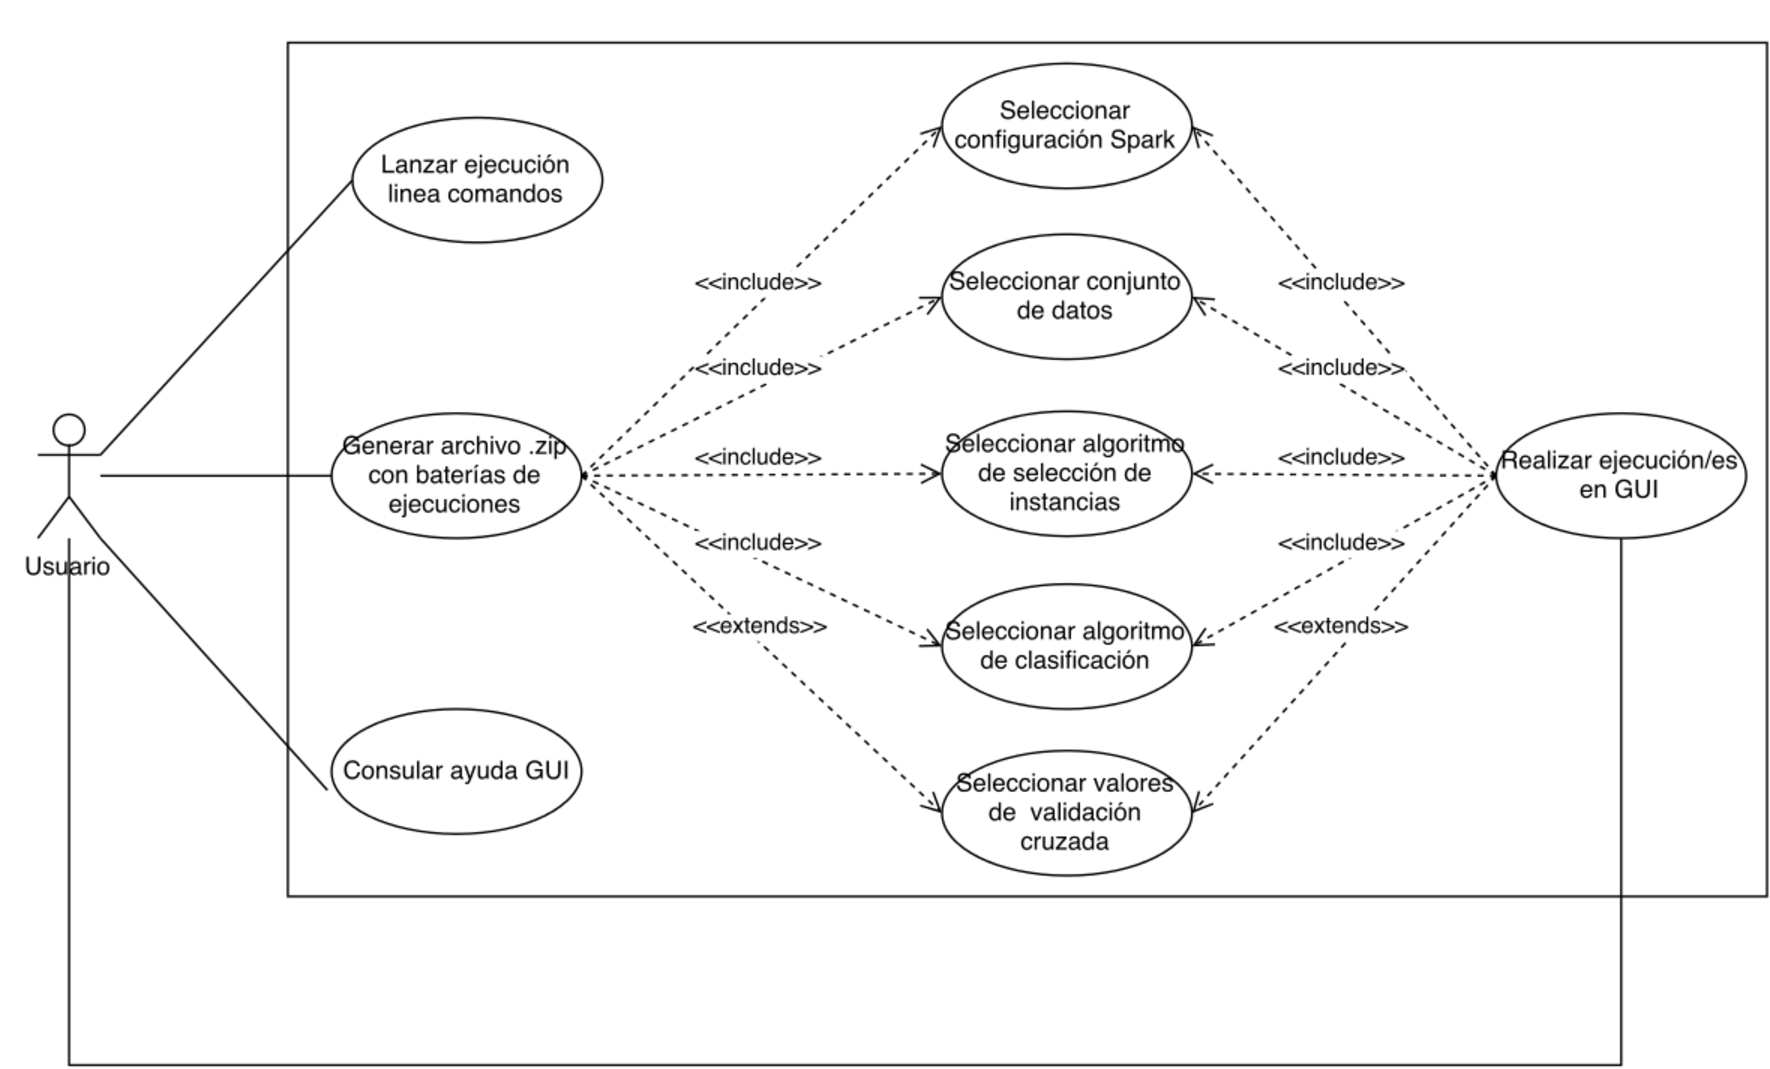
\includegraphics[width=1.0\textwidth]{img/anexo/diagrama_casos_de_uso}
		\caption{Diagrama de casos de uso.}\label{fig:img/anexo/diagrama_casos_de_uso}
	\end{figure}

%\imagen{img/anexo/diagrama_casos_de_uso}{Diagrama de casos de uso.}

 
\subsection{Casos de uso}
 
\begin{table}
  \begin{center}
   \begin{tabular}{|>{\cellcolor[gray]{0.8}} L{3cm} | L{9cm} |}
    \hline
    Caso de uso & Lanzar ejecución - Línea de comandos\\
    \hline
    Versión & 1.0 \\
    \hline
    Autor & Alejandro González Rogel \\
    \hline
    Requisitos & RF-1\newline
		RF-1.1\newline
		RF-1.2\newline
		RF-1.3\newline
		RF-1.4\newline
		RF-1.5\newline
		RF-1.6\\
    \hline
    Descripción & El usuario puede realizar la invocación, por línea de comandos, de un nueva tarea que implique un selector de instancias y un clasificador. Para ello necesitará aportar, además, una lista de parámetros que permitan la configuración de todos los componentes involucrados.\\
    \hline
    Precondiciones & Ninguna \\
    \hline
    Acciones & 1. El usuario realiza el lanzamiento de la aplicación mediante consola de comandos usando el script ``spark-submit'' proporcionado por Spark. \newline
    2. La aplicación realiza la ejecución. \newline
    \hspace{1em} 2.1 Se muestra periodicamente, en mensajes por consola, el punto de la ejecución en el que nos encontramos. \newline
    \hspace{1em} 2.2 La aplicación escribe los resultados de la ejecución en un fichero.\newline
    \hspace{1em} 2.3 La aplicación muestra un último mensaje indicando la correcta ejecución.\\
    \hline
    Postcondiciones & Ningua \\
    \hline
    Excepciones & Los parámetros introducidos en la invocación del programa son erróneos. Se paralizará la ejecución y se informará mediante un mensaje por consola de comandos si este fuese el caso. \\
    \hline
    Importancia & Alta \\
    \hline
   \end{tabular}
   \caption{Caso de uso ``Lanzar ejecución - Línea de comandos''}
   \label{tabla:casoUso1}
  \end{center}
 \end{table} 
 
 
\begin{table}
  \begin{center}
   \begin{tabular}{|>{\cellcolor[gray]{0.8}} L{3cm} | L{9cm} |}
    \hline
    Caso de uso & Realizar ejecución/es GUI\\
    \hline
    Versión & 1.0 \\
    \hline
    Autor & Alejandro González Rogel \\
    \hline
    Requisitos & 
    		RF-2\newline
    		RF-2.1\newline
		RF-2.2\newline
		RF-2.3\newline
		RF-2.4\newline
		RF-2.5\newline
		RF-2.6\\
    \hline
    Descripción & Mediante el uso de la interfaz gráfica, el usuario puede programar una o varias ejecuciones y lanzarlas en el momento.\\
    \hline
    Precondiciones & El usuario ha iniciado la interfaz gráfica. \\
    \hline
    Acciones & 1. El usuario completa los campos de opciones comunes de Spark. \newline
    			   2. El usuario indica una o varias configuraciones de Spark \newline
    			   3. El usuario indica uno o varios conjuntos de datos \newline
    			   4. El usuario selecciona uno o varios selectores de instancias. \newline
    			   5. El usuario selecciona un clasificador. \newline
    			   6. El usuario puede indicar opciones para la validación cruzada (opcional). \newline
    			   7. El usuario presiona un botón para ejecutar las tareas programadas. \newline
    			   8. La aplicación informa cuando se finalice la operación.
    			   \\
    \hline
    Postcondiciones & Los resultados de la ejecución han sido almacenados en un fichero de texto en la ruta correspondiente. \\
    \hline
    Excepciones & Ninguna \\
    \hline
    Importancia & Baja \\
    \hline
   \end{tabular}
   \caption{Caso de uso ``Realizar ejecución/es GUI''}
   \label{tabla:casoUso2}
  \end{center}
 \end{table} 
 
 
\begin{table}
  \begin{center}
   \begin{tabular}{|>{\cellcolor[gray]{0.8}} L{3cm} | L{9cm} |}
    \hline
    Caso de uso & Generar archivo .zip con baterías de ejecuciones\\
    \hline
    Versión & 1.0 \\
    \hline
    Autor & Alejandro González Rogel \\
    \hline
    Requisitos & 
    		RF-2\newline
    		RF-2.1\newline
		RF-2.2\newline
		RF-2.3\newline
		RF-2.4\newline
		RF-2.5\newline
		RF-2.6\\
    \hline
    Descripción & Mediante el uso de la interfaz gráfica, el usuario puede programar una o varias ejecuciones y generar un archivo de extensión .zip que contendrá un script de lanzamiento y todos los conjuntos de datos necesarios para la ejecución.\\
    \hline
    Precondiciones & El usuario ha iniciado la interfaz gráfica. \\
    \hline
    Acciones & 1. El usuario completa los campos de opciones generales de Spark. \newline
    			   2. El usuario indica una o varias configuraciones de Spark \newline
    			   3. El usuario indica uno o varios conjuntos de datos \newline
    			   4. El usuario selecciona uno o varios selectores de instancias. \newline
    			   5. El usuario selecciona un clasificador. \newline
    			   6. El usuario puede indicar opciones para la validación cruzada (opcional). \newline
    			   7. El usuario presiona un botón para generar el archivo zip. \newline
    			   8. La aplicación informa cuando se finalice la operación.
    			   \\
    \hline
    Postcondiciones & Se ha generado un archivo de extensión .zip \\
    \hline
    Excepciones & Ninguna \\
    \hline
    Importancia & Media \\
    \hline
   \end{tabular}
   \caption{Caso de uso ``Generar archivo .zip con baterías de ejecuciones''}
   \label{tabla:casoUso3}
  \end{center}
 \end{table}  
 
 
 \begin{table}
  \begin{center}
   \begin{tabular}{|>{\cellcolor[gray]{0.8}} L{3cm} | L{9cm} |}
    \hline
    Caso de uso & Seleccionar configuración Spark\\
    \hline
    Versión & 1.0 \\
    \hline
    Autor & Alejandro González Rogel \\
    \hline
    Requisitos & RF-2\newline
    				 RF-2.1\newline
    				 RF-3\newline
    				 RF-3.1 \\
    \hline
    Descripción & El usuario puede indicar una configuración de Spark rellenando un conjunto de campos de texto. \\
    \hline
    Precondiciones & El usuario ha iniciado la interfaz gráfica.\\
    \hline
    Acciones & 1. El usuario ha presionado un botón para añadir una nueva configuración de Spark. \newline
    			   2. La aplicación muestra un nuevo diálogo. \newline
    			   3. El usuario rellena todos los campos mostrados en el nuevo diálogo. \newline
    			   4. El usuario presiona un botón para aceptar la nueva configuración.  \\
    \hline
    Postcondiciones & Una nueva configuración ha de haberse añadido a la lista de configuraciones. \\
    \hline
    Excepciones & Ninguna \\
    \hline
    Importancia & Baja \\
    \hline
   \end{tabular}
   \caption{Caso de uso ``Seleccionar configuración Spark''}
   \label{tabla:casoUso5}
  \end{center}
 \end{table}
 
  \begin{table}
  \begin{center}
   \begin{tabular}{|>{\cellcolor[gray]{0.8}} L{3cm} | L{9cm} |}
    \hline
    Caso de uso & Seleccionar conjunto de datos\\
    \hline
    Versión & 1.0 \\
    \hline
    Autor & Alejandro González Rogel \\
    \hline
    Requisitos & RF-2\newline
    				 RF-2.2\newline
    				 RF-3\newline
    				 RF-3.2 \\
    \hline
    Descripción & El usuario puede indicar un fichero que contenga un conjunto de datos así como algunos parámetros que permitan su lectura. \\
    \hline
    Precondiciones & El usuario ha iniciado la interfaz gráfica.\\
    \hline
    Acciones & 1. El usuario ha presionado un botón para añadir un nuevo conjunto de datos. \newline 
    2. La aplicación muestra un nuevo diálogo. \newline
    			   3. El usuario selecciona el botón para buscar en los archivos del sistema un conjunto de datos. Alternativamente, puede escribirlo manualmente. \newline
    			   4. El usuario cumplimenta todos los campos restantes mostrados en el diálogo. \newline
    			   5. El usuario presiona un botón para aceptar la nueva configuración. \\
    \hline
    Postcondiciones & Un nuevo conjunto de datos, junto con sus opciones de lectura, ha de haberse añadido a la lista de conjuntos de datos. \\
    \hline
    Excepciones & Ninguna \\
    \hline
    Importancia & Baja \\
    \hline
   \end{tabular}
   \caption{Caso de uso ``Seleccionar conjunto de datos''}
   \label{tabla:casoUso6}
  \end{center}
 \end{table}
 
 
   \begin{table}
  \begin{center}
   \begin{tabular}{|>{\cellcolor[gray]{0.8}} L{3cm} | L{9cm} |}
    \hline
    Caso de uso & Seleccionar algoritmo de selección de instancias\\
    \hline
    Versión & 1.0 \\
    \hline
    Autor & Alejandro González Rogel \\
    \hline
    Requisitos & RF-2\newline
    				 RF-2.3\newline
    				 RF-3\newline
    				 RF-3.3 \\
    \hline
    Descripción & El usuario puede seleccionar un algoritmo de selección de instancias de entre las posibles opciones y configurarlo para su ejecución. \\
    \hline
    Precondiciones & El usuario ha iniciado la interfaz gráfica.\\
    \hline
    		Acciones & 1.El usuario ha presionado el botón para añadir un nuevo selector de instancias.  \newline
    		
    		2. La aplicación muestra un nuevo diálogo. \newline
    		3. El usuario selecciona, tras pulsar el botón de selección, el filtro que desea. \newline
    		4. La aplicación añade nuevos campos al diálogo.
    		5. El usuario cumplimenta los nuevos campos mostrados en el diálogo. \newline
    		6. El usuario presiona un botón para aceptar la nueva configuración. \\
    \hline
    Postcondiciones & Un nuevo selector de instancias, junto con su configuración, ha de haberse añadido a la lista de conjuntos de datos. \\
    \hline
    Excepciones & Ninguna \\
    \hline
    Importancia & Baja \\
    \hline
   \end{tabular}
   \caption{Caso de uso ``Seleccionar algoritmo de selección de instancias''}
   \label{tabla:casoUso7}
  \end{center}
 \end{table}
 
    \begin{table}
  \begin{center}
   \begin{tabular}{|>{\cellcolor[gray]{0.8}} L{3cm} | L{9cm} |}
    \hline
    Caso de uso & Seleccionar algoritmo de clasificación.\\
    \hline
    Versión & 1.0 \\
    \hline
    Autor & Alejandro González Rogel \\
    \hline
    Requisitos & RF-2\newline
    				 RF-2.4\newline
    				 RF-3\newline
    				 RF-3.4 \\
    \hline
    Descripción & El usuario puede seleccionar un algoritmo de clasificación y configurarlo para su ejecución. \\
    \hline
    Precondiciones & El usuario ha iniciado la interfaz gráfica.\\
    \hline
    		Acciones & 1. El usuario presiona el botón que permite seleccionar entre los diferentes clasificadores posibles. \newline
    		2. El usuario selecciona un clasificador.\newline
    		3. La aplicación genera nuevos campos con las opciones de configuración del clasificador.\newline
    		4. El usuario rellena los campos con las opciones de configuración.    \\ 			
    \hline
    Postcondiciones & Ninguna\\
    \hline
    Excepciones & Ninguna \\
    \hline
    Importancia & Baja \\
    \hline
   \end{tabular}
   \caption{Caso de uso ``Seleccionar algoritmo de clasificación''}
   \label{tabla:casoUso8}
  \end{center}
 \end{table}
 
 
     \begin{table}
  \begin{center}
   \begin{tabular}{|>{\cellcolor[gray]{0.8}} L{3cm} | L{9cm} |}
    \hline
    Caso de uso & Seleccionar valores de validación cruzada.\\
    \hline
    Versión & 1.0 \\
    \hline
    Autor & Alejandro González Rogel \\
    \hline
    Requisitos & RF-2\newline
    				 RF-2.5\newline
    				 RF-3\newline
    				 RF-3.5 \\
    \hline
    Descripción & El usuario puede indicar una configuración de validación cruzada con la que realizar las ejecuciones. \\
    \hline
    Precondiciones & El usuario ha iniciado la interfaz gráfica.\\
    \hline
    		Acciones & 1. El usuario marca la opción que habilita la validación cruzada. \newline
    		2. El usuario cumplimenta los campos de configuración de la validación cruzada.\\
    \hline
    Postcondiciones & Ninguna\\
    \hline
    Excepciones & Ninguna \\
    \hline
    Importancia & Baja \\
    \hline
   \end{tabular}
   \caption{Caso de uso ``Seleccionar valores de validación cruzada''}
   \label{tabla:casoUso9}
  \end{center}
 \end{table}
 
 
 
 \begin{table}
  \begin{center}
   \begin{tabular}{|>{\cellcolor[gray]{0.8}} L{3cm} | L{9cm} |}
    \hline
    Caso de uso & Consultar ayuda GUI\\
    \hline
    Versión & 1.0 \\
    \hline
    Autor & Alejandro González Rogel \\
    \hline
    Requisitos & RF-4 \\
    \hline
    Descripción & El usuario puede consultar el funcionamiento de la interfaz gráfica mediante un botón de ayuda proporcionado en dicha interfaz.\\
    \hline
    Precondiciones & Se ha iniciado la interfaz gráfica. \\
    \hline
    Acciones & 1. El usuario presiona sobre el botón de ayuda en la interfaz. \newline
    				2. La aplicación muestra una nueva ventana con la ayuda.\\
    \hline
    Postcondiciones & Ninguna \\
    \hline
    Excepciones & Ninguna \\
    \hline
    Importancia & Baja \\
    \hline
   \end{tabular}
   \caption{Caso de uso ``Consultar ayuda GUI''}
   \label{tabla:casoUso4}
  \end{center}
 \end{table}